\documentclass{article}

\usepackage{graphicx} % Required for inserting images
\usepackage{verbatim}
\usepackage[utf8]{inputenc}
\usepackage{graphicx}
\usepackage{float}
\usepackage{fancyvrb}
\usepackage{varwidth}
\usepackage{amsmath}
\usepackage{siunitx}
\usepackage{caption}
\usepackage{subcaption}


\title{Foundations of Intelligent and Learning Agents\\CS747}
\author{Mohit\\20D070052 }
\date{September 2023}

\begin{document}

\maketitle
\begin{figure}[H]
\begin{center}

\includegraphics[scale = 0.2]{LOGO.jpeg}
\end{center}
\end{figure}
\section{Student Details}
\begin{tabular}{ l l  }
 Name: & Mohit \\ 
 Roll No: & 20D070052  \\  
\end{tabular}

\newpage

\section{Task 1}


\subsection{UCB Algorithm}
We know that in UCB algorithm the arm to be pulled is selected by :\\

$ucb_a^t = \hat{p}_a^t + \sqrt{2ln(t)/u_a^t}$ \\

Now in the algorithm, Parameters : \\
self.counts - An array which counts the number of times each arm was pulled as per it's index\\
self.values - An array which keeps a track of the rewards that we are getting from each arm\\
self.empmean - An array which keeps a track of the empirical mean of each arm after every pull given by reward for that arm/ number of times that arm was pulled\\
self.time - Keeps a track of the time i.e. mainly the total number of pulls till now \\

Note : We could have removed the empmean and time variables but they help in providing more readability hence they are kept \\

Now the algorithm is mainly in the givepull function :\\
Firstly we initiate 2 variables i.e. maxucb to record the maximum ucb for all arms also index will be that arm which has the maximum ucb. Now initially we will sample each arm once so that $u_a^t$ is non zero for all arms after this. After this we have a loop in which we iterate through all the arms and check which arm has the maximum ucb and return the index corresponding to that arm.\\

Now in the getreward function we update the count of the arm that was pulled, add the reward corresponding to that arm pull, increment the time by 1 and update the empirical mean of that arm.\\



\subsection{Plot}
\begin{figure}[H]
\centering
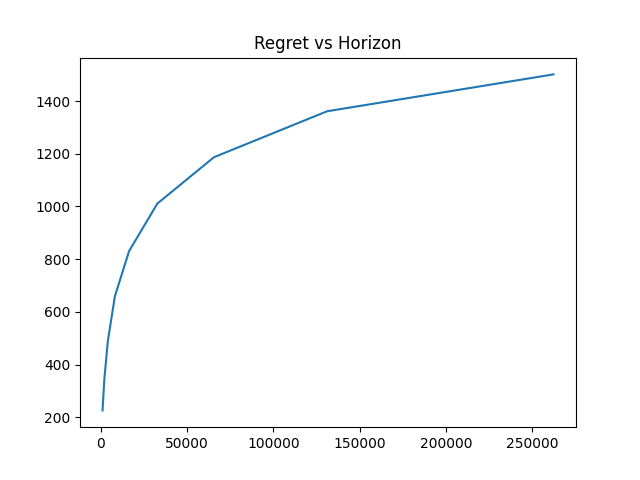
\includegraphics[scale = 0.5]{task1-UCB-20230903-185503.png}
\caption{Regret vs Horizon for UCB Algorithm}
\end{figure}


As expected the regret is logarithmic with respect to the horizon which is much better than the E-Greedy Method.

\subsection{KL-UCB Algorithm}
We know that in KL-UCB algorithm the arm to be pulled is selected by :\\

$ ucbkl_a^t = max{ q \in [ p_a^t,1 ] such that (u_a^t)(KL( p_a^t, q) \leq ln(t) + cln(ln(t)) } , c \geq 3$\\

However in class it was told that c should be $\geq$ 3 but in the paper it is recommended to take c = 0 and testcases are also designed according to that so we will also use the same.\\


Now in the algorithm, Parameters : \\
self.counts - An array which counts the number of times each arm was pulled as per it's index\\
self.values - An array which keeps a track of the rewards that we are getting from each arm\\
self.empmean - An array which keeps a track of the empirical mean of each arm after every pull given by reward for that arm/ number of times that arm was pulled\\
self.time - Keeps a track of the time i.e. mainly the total number of pulls till now \\

Note : We could have removed the empmean and time variables but they help in providing more readability hence they are kept \\

Now in the algorithm is mainly in the givepull function :\\
Firstly we initiate 2 variables i.e. qmax to know that what is the maximum q for any arm till now also index will be that arm which has the maximum q. Now initially we will sample each arm once so that $u_a^t$ is non zero for all arms after this. Now in this algorithm we have used the fact that KL divergence is an increasing function in the variable q so to make the algorithm optimized we will use binary search to reduce time complexity. After this we have a loop in which we iterate through all the arms and for each arm we check the maximum q for which the condition is satisfied and check if that q is greater than qmax then we update the qmax with this q and index with this index. Also we want to run the algorithm to run atleast once so that's why there is a variable of count to count the number of times the loop has run cause there can be a case in which $p_a^t$ is already equal to 1 so we want to include that case also.\\

Now in the getreward function we update the count of the arm that was pulled, add the reward corresponding to that arm pull, increment the time by 1 and update the empirical mean of that arm.\\

\subsection{Plot}

\begin{figure}[H]
\centering
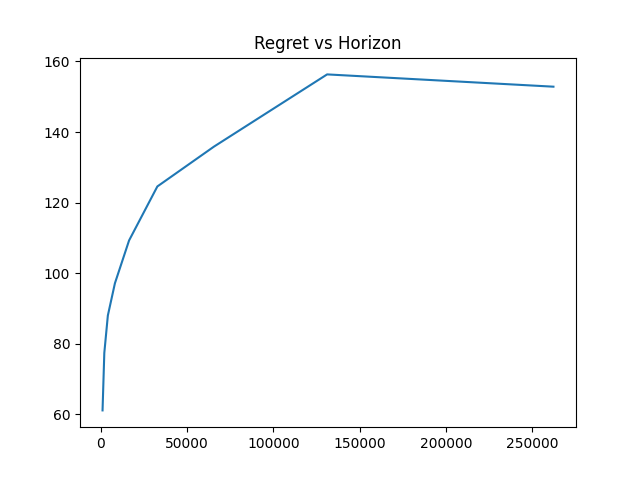
\includegraphics[scale = 0.5]{task1-KL_UCB-20230906-020050.png}
\caption{Regret vs Horizon for KL-UCB Algorithm}
\end{figure}


As expected the regret is logarithmic with respect to the horizon which is much better than the E-Greedy Method. The regret is much better than the UCB algorithm also because KL-UCB gives a much tighter confidence bound than UCB and the regret matches the lower bound. And even the regret decreases because there is a high probability of regret going negative since our expectation is now zero once we reach optimal convergence. The regret seems to be linear in the later part but that is because of the step size of the horizon we are using.



\subsection{Thompson Sampling Algorithm}
We know that in Thompson Sampling Algorithm the arm to be pulled is selected by :\\

Now in the algorithm, Parameters : \\
self.counts - An array which counts the number of times each arm was pulled as per it's index\\
self.values - An array which keeps a track of the rewards that we are getting from each arm\\

Now in the algorithm is mainly in the givepull function :\\
Firstly we initiate 2 variables i.e. the max sample that we have recieved from all arms and index which stores the index of that arm for which we got the max sample. Now initially we will sample each arm once so that . After this we have a loop in which we iterate through all the arms and check which arm has the maximum ucb and return the index corresponding to that arm.\\

Now in the getreward function we update the count of the arm that was pulled and add the reward corresponding to that arm pull.

\subsection{Plot}
\begin{figure}[H]
\centering
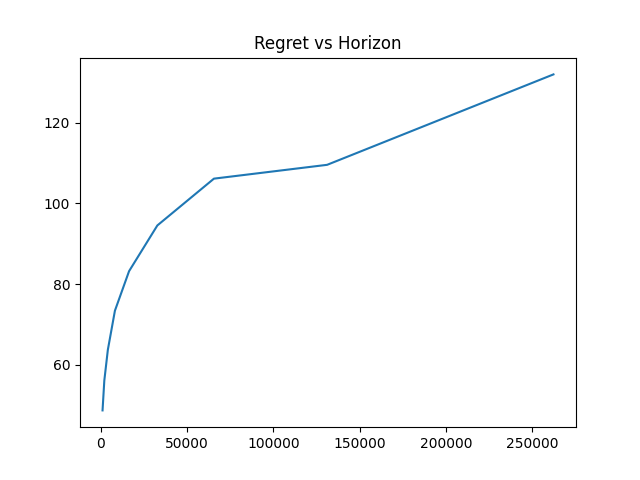
\includegraphics[scale = 0.5]{task1-Thompson_Sampling-20230903-190434.png}
\caption{Regret vs Horizon for Thompson Algorithm}
\end{figure}


As expected the regret is logarithmic with respect to the horizon which is much better than the E-Greedy Method. The regret is much better than the UCB algorithm also because Thompson gives a much tighter confidence bound than UCB and the regret matches the lower bound. The regret seems to be linear in the later part but that is because of the step size of the horizon we are using. We can also observe that the regret for Thompson method is smaller than the KL-UCB hence we will use this in further tasks also like 3 and 4.

\section{Task 2}
This task was divided into 2 parts which are explained below:

\subsection{Task 2a}
In this task we have increased the p2 from 0 to 0.9 in steps of 0.05 over a horizon of 30,000. The results obtained are as listed below in the next sections :

\subsubsection{Plot}

\begin{figure}[H]
\centering
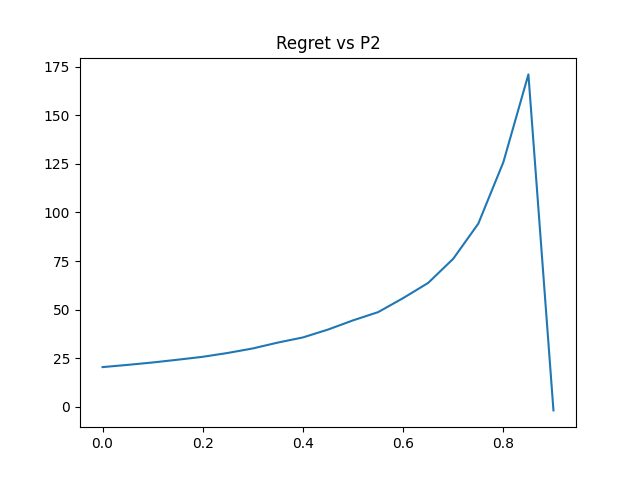
\includegraphics[scale = 0.5]{task2-UCB--20230905-203013.png}
\caption{Regret vs P2 for UCB Algorithm}
\end{figure}

\subsubsection{Observations and Reasoning}
We observe that the regret continues to increase upto a certain point and then abruptly falls to zero. The regret when both probabilities are equal is expected to be zero. Since both the arms have equal probability of reward it doesn't matter which arm we pick so regret has to be zero. The regret continues to increase upto 0.85 and has to be zero at 0.9 because of the step size else it would have increased after 0.85 also.


\subsection{Task 2b}
In this task we have increased the p2 from 0 to 0.9 in steps of 0.05 over a horizon of 30,000 but also we are increasing p1 such that p1 - p2 = 0.1 remains constant. The results obtained are as listed below in the next sections :

\subsubsection{Plots}

\begin{figure}[H]
\centering
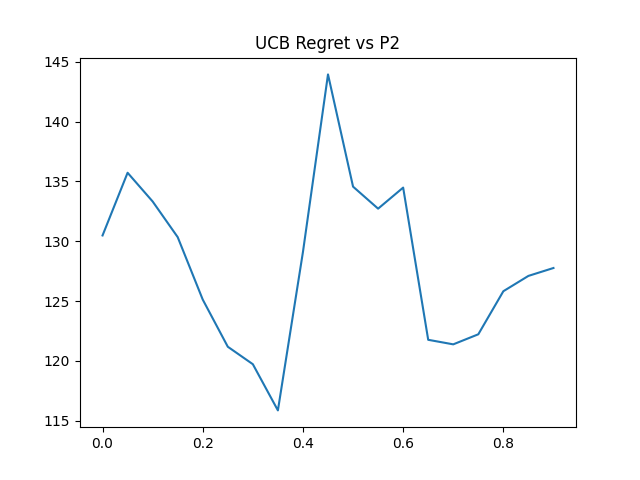
\includegraphics[scale = 0.5]{task2b-UCB--20230906-101751.png}
\caption{Regret vs P2 for UCB Algorithm}
\end{figure}

\begin{figure}[H]
\centering
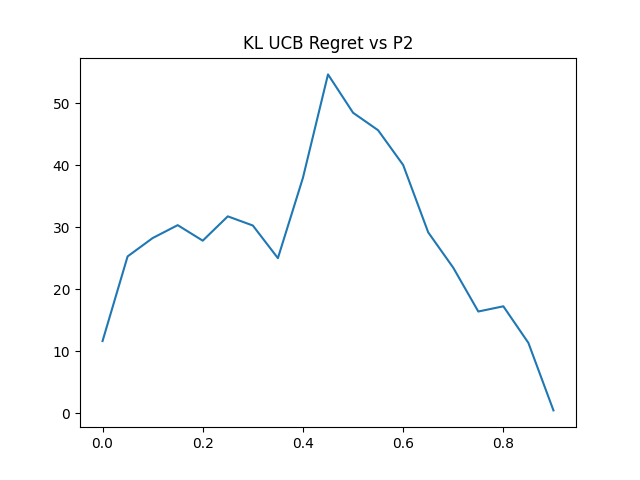
\includegraphics[scale = 0.5]{task2b-KL-UCB-20230906-101751.png}
\caption{Regret vs P2 for KL-UCB Algorithm}
\end{figure}

\subsubsection{Observations and Reasoning}
\begin{itemize}
\item Firstly we can observe that the regret for KL-UCB is less than half of the UCB algorithm and this is expected because as studied in class the KL-UCB gives a much tighter confidence bound than UCB.
\item For both of these algorithms we can observe that the regret maximizes when p2 goes from 0.35 to 0.45 i.e. when p1 goes from 0.45 to 0.55.
\end{itemize}


\section{Task 3}
In this task we were a given that an arm can also give a faulty output.

\subsection{Algorithm}
In this question also we can directly use the Thompson Sampling Method. How the algorithm is implemented is already answered in Task 1. The explanation behind the algorithm is as given below :

\subsection{Plot of Reward vs Horizon}
\begin{figure}[H]
\centering
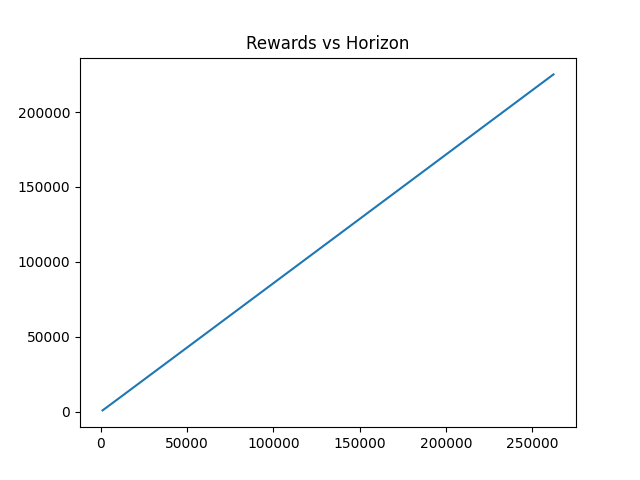
\includegraphics[scale = 0.5]{task3-Faulty-20230906-104650.png}
\caption{Reward vs Horizon for Faulty Bandits Algorithm}
\end{figure}

\subsection{Reasoning Behind Algorithm}
Here it is given that the fault is equal for all arms that if an arm is pulled it gives faulty output. Therefore we can use Thompson Sampling here also because irrespective of the arm that is pulled fault probability is equal hence ideally we would like to follow the optimum method only so that if the fault is not detected then at least we are picking the right arm and if a fault is detected then it will not matter which arm is being pulled hence we will be able to get the best reward through thompson sampling. Also there is one rare case in which this algorithm can fail and that is when the arm with maximum probability of reward (greater than 0.5 i.e. the fault reward) gives faulty reward everytime and thus affecting its beta distribution to make it below a less optimal arm however this is quite rare because other arms also will have the same problem and hence net effect can be ignored and we can assume that the arm with maximum probability will still be largest. This algorithm can fail if each arm has different probability of faults but here it is not the case hence the algorithm works and reward is also linear with regret. 

\section{Task 4}
In this task we were dealing with 2 bandit instances at once and arm for each of the bandit could be pulled randomly.

\subsection{Algorithm}
In this question also we can directly use the Thompson Sampling Method. How the algorithm is implemented is already answered in Task 1. The explanation behind the algorithm is as given below :

\subsection{Plot of Reward vs Horizon}
\begin{figure}[H]
\centering
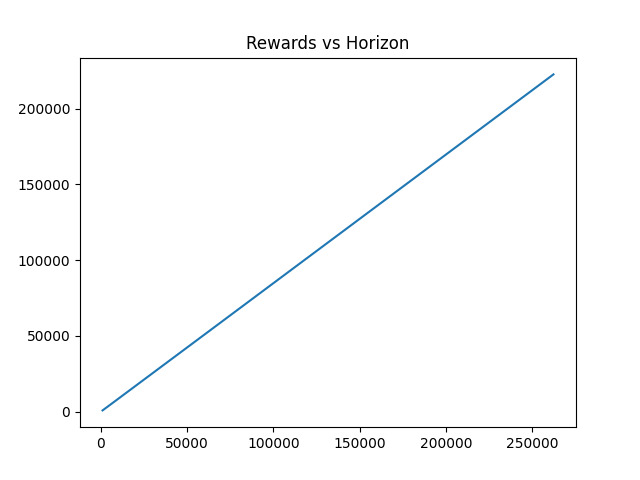
\includegraphics[scale = 0.5]{task4-Multi Bandit-20230906-124339.png}
\caption{Reward vs Horizon for Multi-Bandit Algorithm}
\end{figure}

\subsection{Reasoning Behind Algorithm}
In Thompson sampling we take a random sample from the beta distribution of each arm, since the probability of selecting each arm is 0.5 due to uniform choice of bandit. So if we combine both of these bandit instances we can have a joint probability distribution of each arm and select the sample of maximum value after this it won't matter which bandit instance is chosen cause we are taking both of these instances together. Otherwise we could have used 2 separate thompson sampling arrays for each bandit instance, select samples from beta distributions, and sort both of these arrays in increasing order along with the arm for which they are observed. Now we can select that arm which appears in both of these arrays in the initial part so that whichever bandit gets selected we get better reward. However this approach seemed computationally heavy and directly using the first method works with a linear reward hence that method was used.


\end{document}